\documentclass[]{beamer}
\usepackage[T1]{fontenc}
\usepackage[utf8]{inputenc}
\usepackage{lmodern}
\usepackage[italian]{babel}
\usepackage{mathrsfs}

\title{Le equazioni di Maxwell e le onde elettromagnetiche}
\author{\texorpdfstring{Mattia Cozzi\newline\href{mailto:cozzimattia@gmail.com}{\texttt{cozzimattia@gmail.com}}}{Mattia Cozzi}}
\date{a.s.~2023/2024}

%\documentclass[handout]{beamer}     %usare questa classe per generare l'handout
%\usepackage{pgfpages}   %per mostrare più quadri nella stessa pagina
%\pgfpagesuselayout{4 on 1}[a4paper,border shrink=5mm,landscape]
\usetheme{Singapore}
%\useoutertheme[left]{sidebar} %elementi intorno alle diapositive
\setbeamercovered{dynamic} %modifica l'aspetto del testo grigetto delle diapositive future. Argomenti: invisible/transparent/dynamic
\usecolortheme{orchid}
%COLORE PRINCIPALE
% \definecolor{marroncino}{RGB}{156, 26, 0} % UBC Blue (primary)
% \setbeamercolor{structure}{fg=marroncino} % itemize, enumerate, etc

\theoremstyle{plain}
\newtheorem{teorema}{Teorema}

\usepackage{tikz}
\usepackage{circuitikz}

\usepackage{pgf,pgfplots,graphicx}
\usetikzlibrary{angles,quotes,arrows,shapes,decorations.markings}
\pgfplotsset{compat=1.15}
\usepgfplotslibrary{units,fillbetween} % to add units easily to axis

\newcommand{\fem}{f_{em}}

\def\angolo[#1](#2)(#3:#4:#5)% Syntax: [draw options] (center) (initial angle:final angle:radius)
    { \draw[#1] ($(#2)+({#5*cos(#3)},{#5*sin(#3)})$) arc (#3:#4:#5); }


\begin{document}

\begin{frame}
  \titlepage
\end{frame}





\begin{frame}
\frametitle{Contenuti}
\tableofcontents
\end{frame}


\section{Circuitazione di $ \vec{E}_{ind} $}

\begin{frame}
\frametitle{Campo magnetico e campo elettrico indotto}
\alert<1>{Una corrente indotta è}, come ogni corrente, \alert<1>{uno spostamento di cariche causato da un campo elettrico}.

~\pause

Chiamiamo il campo elettrico generato dai fenomeni induttivi \emph{campo elettrico indotto} $ \vec{E}_{ind} $.

~\pause

Sappiamo che tale $ \vec{E}_{ind} $ è generato da un campo magnetico che varia nel tempo, e \alert<3>{proviamo a caratterizzare $ \vec{E}_{ind} $ mediante la sua circuitazione}, studiando il moto di una carica $ q $ in una spira $ \mathscr{L} $.
\end{frame}


\begin{frame}
\frametitle{Circuitazione di $ \vec{E}_{ind} $ (1)}
Sappiamo che la $ \fem $ è definita come $ \dfrac{L}{q} $, dove $ L $ è il lavoro fatto dalle forze induttive per spostare $ q $ lungo $ \mathscr{L} $.

~\pause

Chiamiamo $ \Delta L_i $ il lavoro compiuto  dalla forza $ \vec{F}_i $ lungo il tratto $ \Delta\vec{\ell}_i $ di $ \mathscr{L} $.\pause
\begin{center}
$ \fem = \dfrac{L}{q} = \dfrac{\sum\limits_{i=1}^n L_i}{q} = \dfrac{\sum\limits_{i=1}^n \vec{F}_i \cdot \Delta\vec{\ell}_i }{q} = \sum\limits_{i=1}^n \dfrac{ \vec{F}_i }{q} \cdot \Delta\vec{\ell}_i $
\end{center}

~\pause

\alert<4>{$ \dfrac{ \vec{F}_i }{q} $ è il campo elettrico $ \vec{E}_i $ che agisce sul tratto $ \Delta\vec{\ell}_i $}, e pertanto la circuitazione compare nella nostra espressione:
\begin{center}
$ \fem = \sum\limits_{i=1}^n \vec{E}_i \cdot \Delta\vec{\ell}_i = \Gamma_\mathscr{L} (\vec{E}) $
\end{center}
\end{frame}

\begin{frame}
\frametitle{Circuitazione di $ \vec{E}_{ind} $ (2)}
La legge di FNL afferma che $ \fem = - \dfrac{d\Phi_S(\vec{B})}{dt} $ e pertanto
\begin{center}
\colorbox{blue!30}{$ \Gamma_\mathscr{L} (\vec{E}) =  - \dfrac{d\Phi_S(\vec{B})}{dt}$}
\end{center}\pause


\begin{alertblock}{Convenzioni!}
La variazione di flusso deve essere calcolata attraverso una qualunque superficie $ S $ che abbia per contorno la curva $ \mathscr{L} $, lungo la quale si calcola la circuitazione.\pause

Il verso di percorrenza di $ \mathscr{L} $ e l'orientazione di $ S $ devono essere legati dalla regola della mano destra: avvolgendo le dita della mano destra nel verso di $ \mathscr{L} $, il pollice indica il verso positivo di $ S $.

\end{alertblock}
\end{frame}






\begin{frame}
\frametitle{Esercizio}
\begin{exampleblock}{Calcolo della circuitazione}
\small{
Una spira circolare di raggio $ 2,9 \, cm $ è immersa in un campo magnetico uniforme di valore $ 6,8 \times 10^{-6} \, T $, le cui linee formano un angolo di $ 60^\circ $ con il piano della spira.  
  \begin{itemize}
    \item Determina il modulo della circuitazione di $ \vec{E} $ lungo un cammino che coincide con la spira circolare.\hspace*{\fill}[$ 0 \, Nm/C = 0 \, V $]
  \end{itemize}
  A partire dall'istante $ t = 0 \, s $, il valore del campo magnetico diminuisce progressivamente fino a raggiungere l'intensità di $ 9,7 \times 10^{-7} \, T $ all'istante $ t_1 = 15 \, s $.
  \begin{itemize}
    \item Determina il modulo della circuitazione media di $ \vec{E} $ lungo un cammino che coincide con la spira circolare durante l'intervallo di tempo in cui il campo magnetico diminuisce di valore.\hspace*{\fill}[$ 9,0 \times 10^{-10} \, Nm/C $]
  \end{itemize}
  }
\end{exampleblock}
\end{frame}










\section{Maxwell}


\begin{frame}
  \frametitle{Nuove formule}
  \begin{block}{Osservazione}
 Con la scoperta dell'induzione elettromagnetica si modifica $ \Gamma_\mathscr{L} (\vec{E}) = 0 $, scrivendola come $ \Gamma_\mathscr{L} (\vec{E}) = - \dfrac{d\Phi_S(\vec{B})}{dt} $. 
\end{block}\pause

~

\begin{alertblock}{Domanda}
Dovremo allora cambiare anche il teorema di Ampère, per cui $ \Gamma_\mathscr{L} (\vec{B}) = \mu_0 \sum\limits_{k=1}^n i_k $?  
\end{alertblock}
\end{frame}

\begin{frame}
\frametitle{James Clerk Maxwell}
\begin{columns}
\begin{column}{0.2\textwidth}
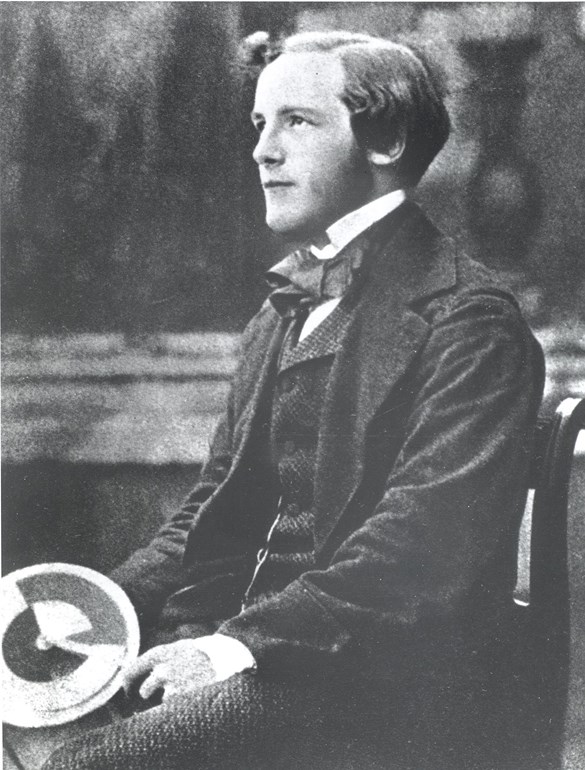
\includegraphics[width=\columnwidth]{img/maxwell.jpg}
\end{column}
\begin{column}{0.7\textwidth}
\begin{itemize}
\item<1-> 1861: James Clerk Maxwell pubblica \emph{On Physical Lines of Force};
\item<2-> 1873: Maxwell pubblica \emph{Treatise On Electricity and Magnetism}, in cui dimostra che \alert<2>{tutte le proprietà elettriche, magnetiche e induttive possono essere derivate da sole quattro equazioni}, che fungono da \alert<2>{assiomi} della teoria;
\item<3-> Maxwell corregge, con originale intuizione, il teorema di Ampère.
\end{itemize}
\end{column}
\end{columns}
\end{frame}


\begin{frame}
  \frametitle{Una situazione}
  Immaginiamo un condensatore che si sta caricando perché collegato a dei fili in cui scorre una corrente $ i $ e calcoliamo le circuitazioni lungo diversi cammini.\pause
\visible<2->{\begin{figure}
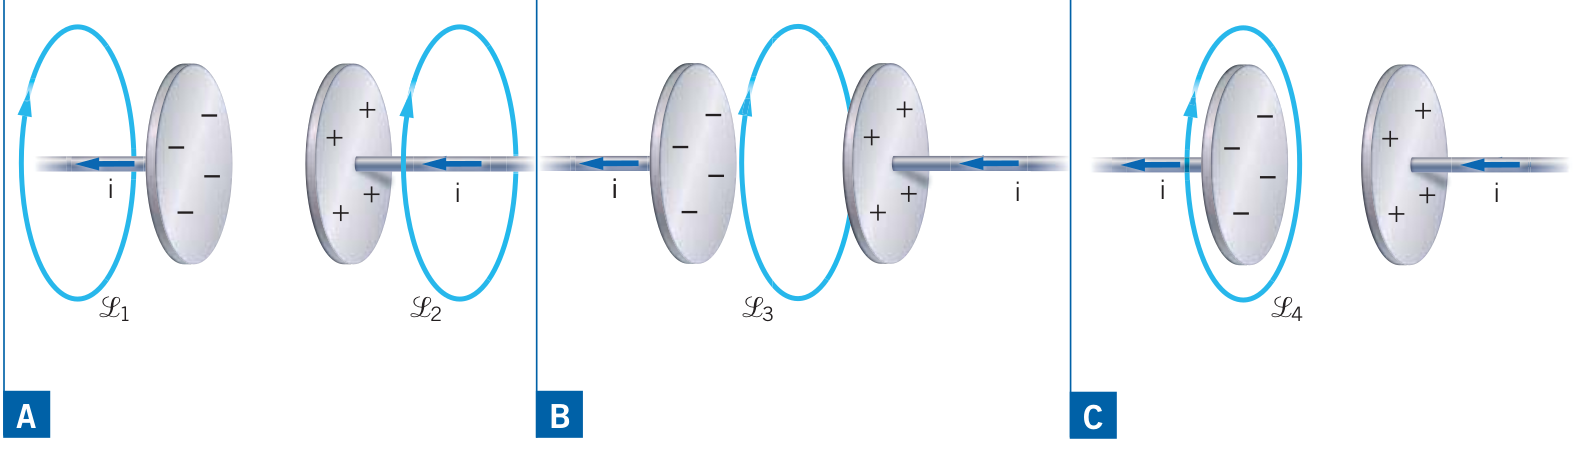
\includegraphics[width=\columnwidth]{img/correntedispostamento.png}
\end{figure}
  
\begin{columns}
\begin{column}{0.33\textwidth}
{\footnotesize La circuitazione lungo $ \mathscr{L}_1 $ e $ \mathscr{L}_2 $ vale $ \mu_0 i $.}
\end{column}
\begin{column}{0.33\textwidth}
{\footnotesize La circuitazione lungo $ \mathscr{L}_3 $ vale zero.}
\end{column}
\begin{column}{0.33\textwidth}
{\footnotesize Quanto vale la circuitazione lungo $ \mathscr{L}_4 $?}
\end{column}
\end{columns}}
\end{frame}




\begin{frame}
  \frametitle{Un problema}
  \begin{figure}
  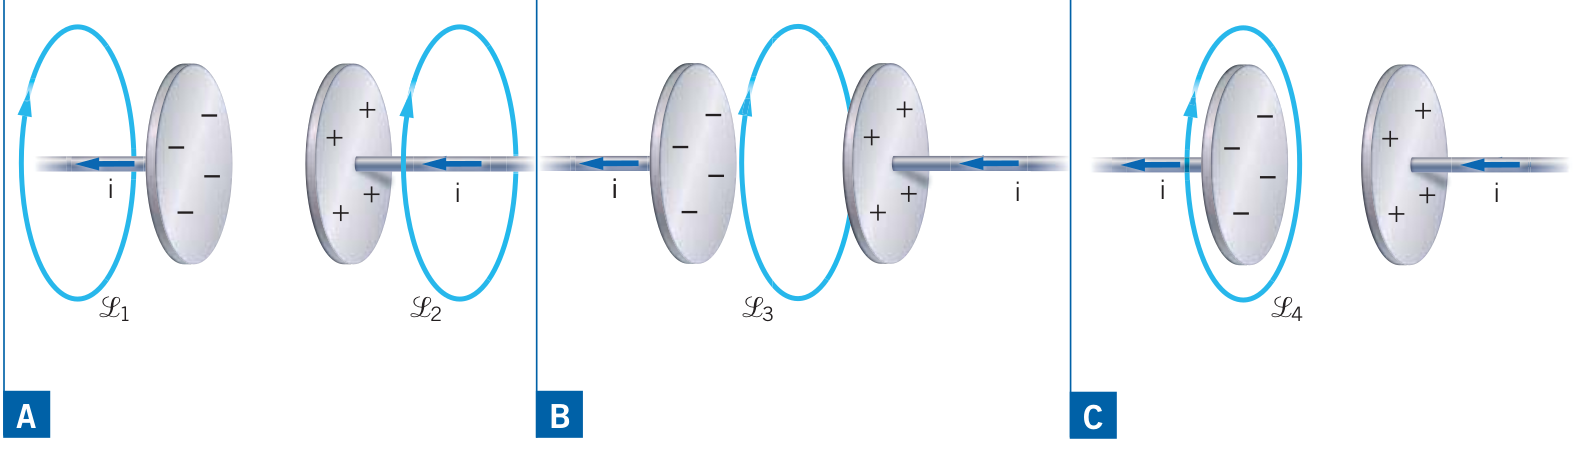
\includegraphics[width=\columnwidth]{img/correntedispostamento.png}
  \end{figure}
  \begin{columns}
\begin{column}{0.33\textwidth}
\begin{center}
{\footnotesize $ \Gamma_\mathscr{L} =  \mu_0 i $}
\end{center}
\end{column}
\begin{column}{0.33\textwidth}
\begin{center}
{\footnotesize $ \Gamma_\mathscr{L} =  0 $}
\end{center}
\end{column}
\begin{column}{0.33\textwidth}
\begin{center}
{\footnotesize $ \Gamma_\mathscr{L} =  ? $}
\end{center}
\end{column}
\end{columns}
~\\~\\
Ci troviamo in una situazione quantomeno strana, con una circuitazione che diventa improvvisamente uguale zero ed è indeterminata al bordo.
\end{frame}





\begin{frame}
  \frametitle{La corrente di spostamento (1)}
  Sappiamo che, grazie alla corrente $ i $, \alert<1>{della carica si accumula sulle piastre del condensatore}, secondo la relazione:
  \begin{center}
  $ i = \dfrac{dq}{dt} $
  \end{center}\pause
  
  Scegliamo ora come \alert<2>{superficie} quella \alert<2>{delimitata da $ \mathscr{L}_4 $} e chiudiamola a nostro piacimento in modo che sia gaussiana.\\~\pause\\  
  Poiché tra le piastre del condensatore si genera un campo elettrico $ \vec{E} $, avremo un certo \alert<3>{flusso che attraversa la superficie}:
  \begin{center}
  $ \Phi_S(\vec{E}) = \dfrac{q}{\varepsilon_0} $~~~~~ovvero~~~~~$ q = \varepsilon_0 \Phi_S(\vec{E}) $
  \end{center}
\end{frame}

\begin{frame}
  \frametitle{La corrente di spostamento (2)}
  Dalle relazioni precedenti otteniamo:
  \begin{center}
  $ i = \varepsilon_0 \dfrac{d\Phi_S(\vec{E})}{dt} $
  \end{center}\pause
  Tale quantità ha le stesse dimensioni e valore della corrente $ i $, ma \alert<2>{non è determinata dal passaggio di carica tra le piastre} (il circuito è aperto), \alert<2>{bensì dalla variazione del flusso del campo elettrico tra di esse}.\\~\pause\\
Maxwell chiamò questo termine \alert<3>{corrente di spostamento $ i_s $}:
  \begin{center}
  \colorbox{blue!30}{$ i_s = \varepsilon_0 \dfrac{d\Phi_S(\vec{E})}{dt} $}
  \end{center}
\end{frame}


\begin{frame}
\frametitle{Il teorema di Ampère-Maxwell}
Maxwell si rende conto che anche \alert{$ i_s $ deve essere presa in considerazione nel teorema di Ampère} e ottiene quello che sarà chiamato teorema di Ampère-Maxwell.
\begin{center}
\colorbox{blue!30}{$ \Gamma_\mathscr{L} (\vec{B}) = \mu_0 (i+i_s) \pause = \mu_0 \left( i + \varepsilon_0 \dfrac{d\Phi_S(\vec{E})}{dt} \right) $}
\end{center}\pause

~

Per il calcolo della circuitazione e del flusso, valgono le stesse osservazioni fatte per la legge di FNL.
\end{frame}



\begin{frame}
\frametitle{Vantaggi della corrente di spostamento}
\begin{figure}
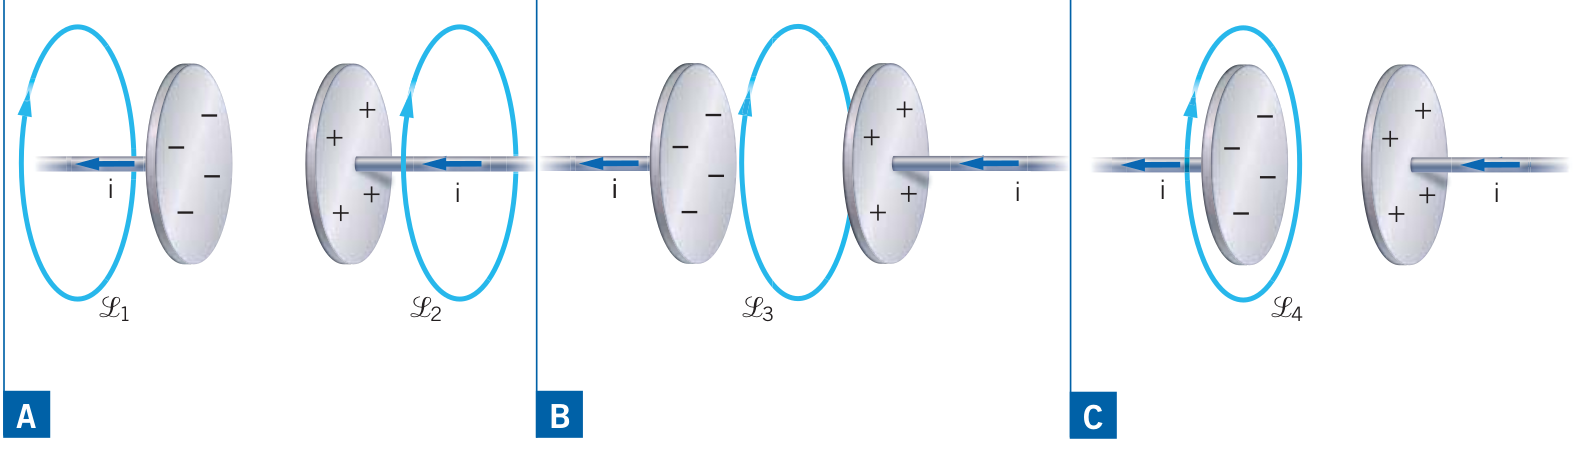
\includegraphics[width=\columnwidth]{img/correntedispostamento.png}
\end{figure}
\begin{center}
$ \Gamma_\mathscr{L} (\vec{B}) = \mu_0 \left( i + \varepsilon_0 \dfrac{d\Phi_S(\vec{E})}{dt} \right) $
\end{center}
Aggiungendo $ i_s $, la circuitazione lungo il cammino $ \mathscr{L}_3 $ ha lo stesso valore di quella lungo $ \mathscr{L}_1 $ e $ \mathscr{L}_2 $, così come quella lungo $ \mathscr{L}_4 $.\\\pause~\\Inoltre, dal teorema di Ampère-Maxwell risulta che \alert{un campo elettrico variabile genera un campo magnetico}.
\end{frame}











\section{Equazioni (2)}

\begin{frame}
\frametitle{Le equazioni di Maxwell (caso generale)}
  Le \alert{equazioni di Maxwell} per il caso generale saranno:\begin{enumerate}
  \item Teorema di Gauss per il campo elettrico
  \begin{center}
  \colorbox{blue!30}{$ \Phi_S (\vec{E}) = \dfrac{Q_{tot}}{\varepsilon_0} $}
  \end{center}\pause
  \item Teorema di Gauss per il campo magnetico
  \begin{center}
  \colorbox{blue!30}{$ \Phi_S (\vec{B}) = 0 $}
  \end{center}\pause
  \item Legge di Faraday-Neumann-Lenz
  \begin{center}
\colorbox{blue!30}{  $ \Gamma_\mathscr{L} (\vec{E}) = -\dfrac{d\Phi_S(\vec{B})}{dt} $}
  \end{center}\pause
  \item Teorema di Ampère-Maxwell
  \begin{center}
  \colorbox{blue!30}{$ \Gamma_\mathscr{L} (\vec{B}) = \mu_0 \left( i + \varepsilon_0 \dfrac{d\Phi_S(\vec{E})}{dt} \right) $}
  \end{center}
\end{enumerate}
\end{frame}



\begin{frame}
  \frametitle{1.~Il teorema di Gauss per $ \vec{E} $}
    \begin{center}
  \colorbox{blue!30}{$ \Phi_S (\vec{E}) = \dfrac{Q_{tot}}{\varepsilon_0} $}
  \end{center}\pause
  Dice che:
  \begin{itemize}
    \item le linee del campo elettrico possono essere aperte;\pause
    \item esistono cariche elettriche isolate;\pause
    \item le cariche sono le sorgenti del campo elettrico.
  \end{itemize}
\end{frame}

\begin{frame}
  \frametitle{2.~Il teorema di Gauss per $ \vec{B} $}
    \begin{center}
  \colorbox{blue!30}{$ \Phi_S (\vec{B}) = 0 $}
  \end{center}\pause
  Dice che:
  \begin{itemize}
    \item per ogni linea di campo entrante c'è una linea di campo uscente, ovvero tutte le linee del campo magnetico sono chiuse;\pause
    \item non esistono poli magnetici isolati.
  \end{itemize}
\end{frame}

\begin{frame}
  \frametitle{3.~La legge di Faraday-Neumann-Lenz}
  \begin{center}
\colorbox{blue!30}{  $ \Gamma_\mathscr{L} (\vec{E}) = -\dfrac{d\Phi_S(\vec{B})}{dt} $}
  \end{center}\pause
  Dice che:
  \begin{itemize}
    \item un campo magnetico variabile è sorgente di un campo elettrico.\pause
    \item il campo elettrico è conservativo solo se è statico.
  \end{itemize}
\end{frame}

\begin{frame}
  \frametitle{4.~Il teorema di Ampère-Maxwell}
  \begin{center}
\colorbox{blue!30}{$ \Gamma_\mathscr{L} (\vec{B}) = \mu_0 \left( i + \varepsilon_0 \dfrac{d\Phi_S(\vec{E})}{dt} \right) $}
  \end{center}\pause
  Dice che:
  \begin{itemize}
    \item il campo magnetico non è conservativo;\pause
    \item le cariche in moto (le correnti) e i campi elettrici variabili sono le sorgenti del campo magnetico.
  \end{itemize}
\end{frame}


\section{Onde}

\begin{frame}
  \frametitle{Il campo elettromagnetico}
Nelle ultime due equazioni \alert<1>{compaiono sia $ \vec{E} $ sia $ \vec{B} $}:{\pause} non è più possibile studiare i due campi separatamente; essi risultano essere \alert<2>{due aspetti di un unico fenomeno}:\pause

~

\begin{block}{Campo elettromagnetico}
Il campo elettrostatico e il campo magnetico sono solo casi particolari del campo elettromagnetico; si ottengono, rispettivamente, soltanto se si hanno cariche ferme oppure correnti continue.
\end{block}
\end{frame}






\begin{frame}
  \frametitle{Propagazione dei campi}
  Se facciamo oscillare una carica in una certa zona dello spazio (ad esempio mediante una \emph{corrente alternata}) otteniamo un \alert<1>{campo elettrico variabile},{\pause} che genera un \alert<2>{campo magnetico variabile},{\pause} che induce un \alert<3>{campo elettrico variabile},{\pause} che genera un \alert<4>{campo magnetico variabile}, ecc.\\\pause~\\Ciò che si ottiene è un'\alert<5>{onda elettromagnetica}, una propagazione ondulatoria del campo elettromagnetico.
\end{frame}



\begin{frame}
  \frametitle{Onde elettromagnetiche}
  Le onde elettromagnetiche:
  \begin{itemize}
    \item furono previste da Maxwell nel 1861 a partire dalle sue equazioni differenziali e dimostrate sperimentalmente da Heinrich Rudolph Hertz nel 1889;\pause
    \item non richiedono un mezzo materiale e si propagano anche nel vuoto;\pause
    \item si muovono nel vuoto a velocità:
    \begin{center}
    $ c = \dfrac{1}{\sqrt{\varepsilon_0 \mu_0}} = 2,998 \times 10^8 \, \frac{m}{s} $
    \end{center}
    e hanno come caso particolare la luce.
  \end{itemize}
\end{frame}


\begin{frame}
  \frametitle{Profilo spaziale delle onde}
  Nelle onde elettromagnetiche i valori oscillanti dei due campi sono legati dalla relazione:
  \begin{center}
  $ E = cB $
  \end{center}
  ed essi oscillano su \emph{piani perpendicolari} tra loro e alla direzione di propagazione dell'onda.\pause
  \begin{figure}
    \begin{tikzpicture}[x={(-10:1cm)},y={(90:1cm)},z={(210:1cm)},scale=.8]
    % Axes
    \draw (-1,0,0) node[above] {$x$} -- (5,0,0);
    \draw (0,0,0) -- (0,2,0) node[above] {$y$};
    \draw (0,0,0) -- (0,0,2) node[left] {$z$};
    % Propagation
    \draw[->, thick] (5,0,0) -- node[above] {$c$} (6,0,0);
    % Waves
    \draw[red,thick] plot[domain=0:4.5,samples=200] (\x,{cos(deg(pi*\x))},0);
    \draw[blue,thick] plot[domain=0:4.5,samples=200] (\x,0,{cos(deg(pi*\x))});
    % Arrows
    \foreach \x in {0.1,0.3,...,4.4} {
      \draw[->,help lines] (\x,0,0) -- (\x,{cos(deg(pi*\x))},0);
      \draw[->,help lines] (\x,0,0) -- (\x,0,{cos(deg(pi*\x))});
    }
    % Labels
    \node[above right] at (0,1,0) {$\vec{E}$};
    \node[below] at (0,0,1) {$\vec{B}$};
  \end{tikzpicture}
  \end{figure}
\end{frame}

\begin{frame}
  \frametitle{Frequenza e lunghezza d'onda}
  Essendo la velocità dell'onda costante nel vuoto, la frequenza delle oscillazioni e la lunghezza d'onda sono inversamente proporzionali secondo la relazione:
   \begin{center}
   $ c = \lambda f \qquad \Longrightarrow \qquad $\colorbox{blue!30}{$ f = \dfrac{c}{\lambda} $}
   \end{center}
\end{frame}


\begin{frame}
\frametitle{Velocità in un mezzo materiale}
  Dato un mezzo materiale di costante dielettrica relativa $ \varepsilon_r $ e permeabilità magnetica relativa $ \mu_0 $, la velocità di un'onda elettromagnetica in quel mezzo sarà:
  \begin{center}
    \colorbox{blue!30}{$ v = \dfrac{1}{\sqrt{\varepsilon_0 \varepsilon_r \cdot \mu_0 \mu_r}} $}
  \end{center}
  o equivalentemente, ponendo $ \varepsilon = \varepsilon_r \varepsilon_0 $ e $ \mu = \mu_r \mu_0 $
  \begin{center}
    \colorbox{blue!30}{$ v = \dfrac{1}{\sqrt{\varepsilon \cdot \mu}} $}
  \end{center}
\end{frame}





\begin{frame}
\frametitle{Esercizio}
\begin{exampleblock}{Onde elettromagnetiche nella materia}
\small{
Un'onda elettromagnetica piana ha frequenza $ 3,0 \, MHz $ e il suo campo elettrico ha un'ampiezza $ E_0 = 3,0 \times 10^{3} \, N/C $. L'onda si propaga in una sostanza che ha permeabilità magnetica relativa di valore $ \mu_r = 1,0 $ e costante dielettrica relativa di valore $ \varepsilon_r = 3,5 $.

Calcola:
  \begin{itemize}
    \item l'ampiezza del campo magnetico;\hspace*{\fill}[$ 1,0 \times 10^{-5} \, T $]
    \item la velocità di propagazione dell'onda piana nella sostanza;\hspace*{\fill}[$ 1,6 \times 10^{8} \, m/s $]
    \item la sua lunghezza d'onda.\hspace*{\fill}[$ 53 \, m $]
  \end{itemize}
  }
\end{exampleblock}
\end{frame}



\section{Spettro}

\begin{frame}
\frametitle{Frequenze e lunghezze d'onda diverse}
  Ciò che distingue un'onda elettromagnetica da un'altra è la sua frequenza (e di conseguenza la sua lunghezza d'onda).\\\pause~\\
  \begin{block}{Spettro elettromagnetico}
    Lo spettro elettromagnetico è l'insieme delle frequenze delle onde elettromagnetiche.
  \end{block}\pause
  
  ~
  
  In particolare, la \alert{luce visibile} è un'onda elettromagnetica con lunghezza d'onda tra $ 7 \times 10^{-7} \, m = 700 \, nm $ (rosso) e $ 4 \times 10^{-7} \, m = 400 \, nm $ (violetto).
\end{frame}


\begin{frame}
\frametitle{Lo spettro elettromagnetico}
  \begin{figure}
  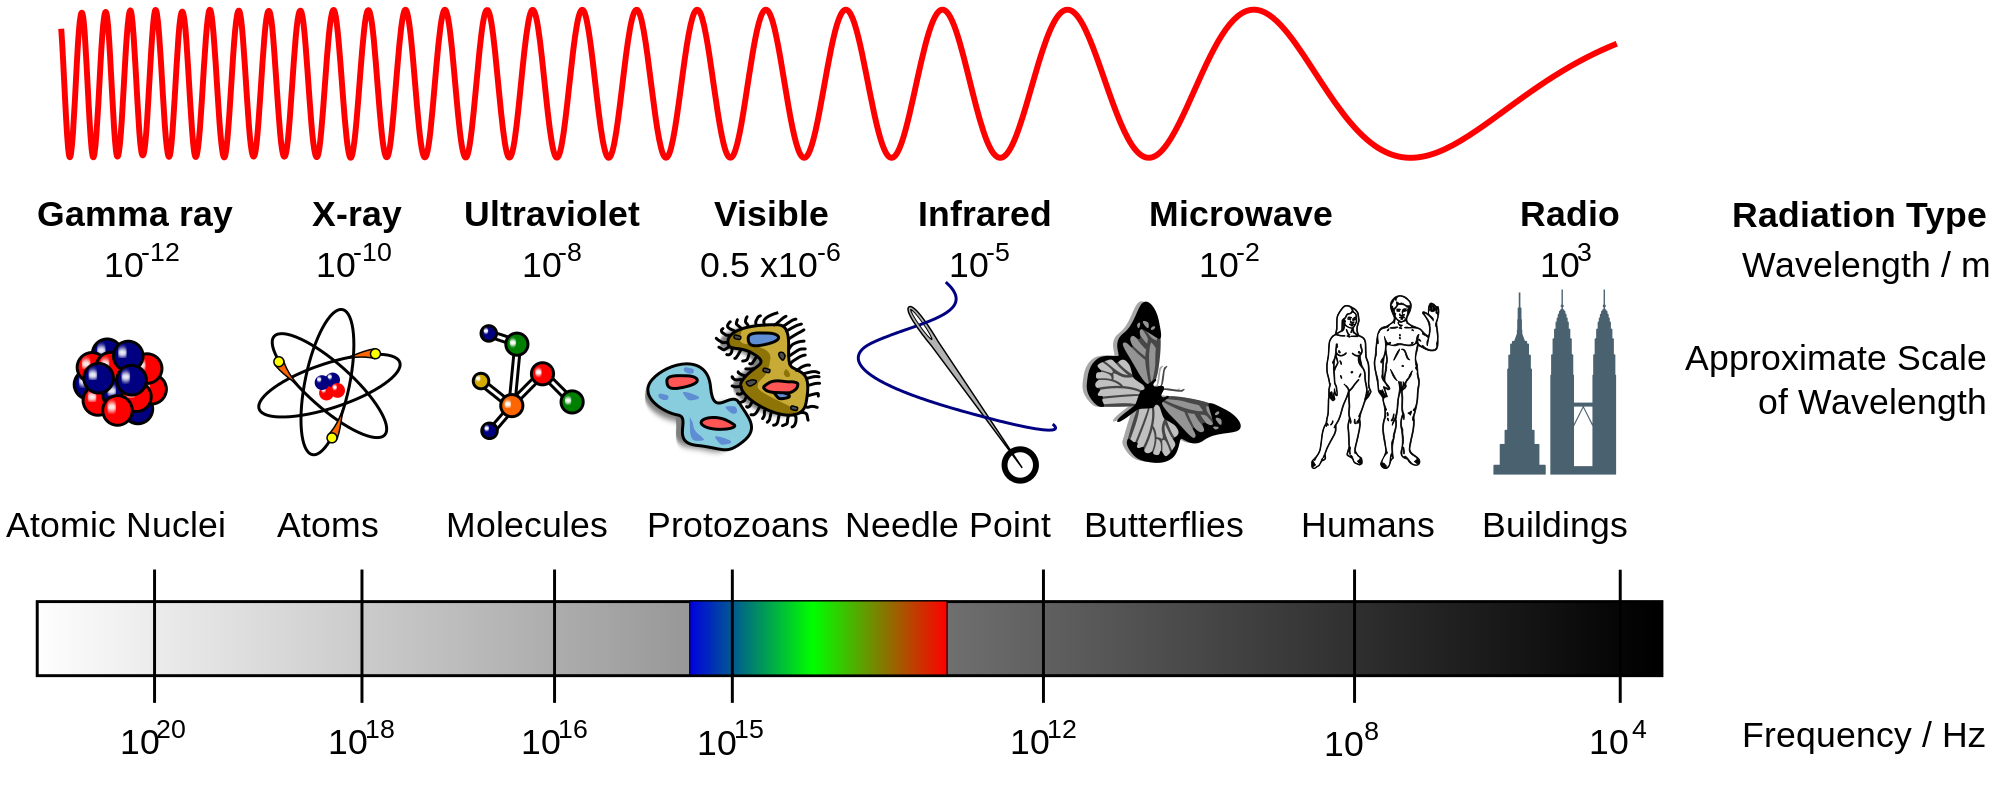
\includegraphics[width=\columnwidth]{img/spettroem.png}
  \end{figure}
\end{frame}



\begin{frame}
\frametitle{Tipi di onde (1)}
  \begin{columns}
    \begin{column}{0.3\textwidth}
      \begin{figure}
        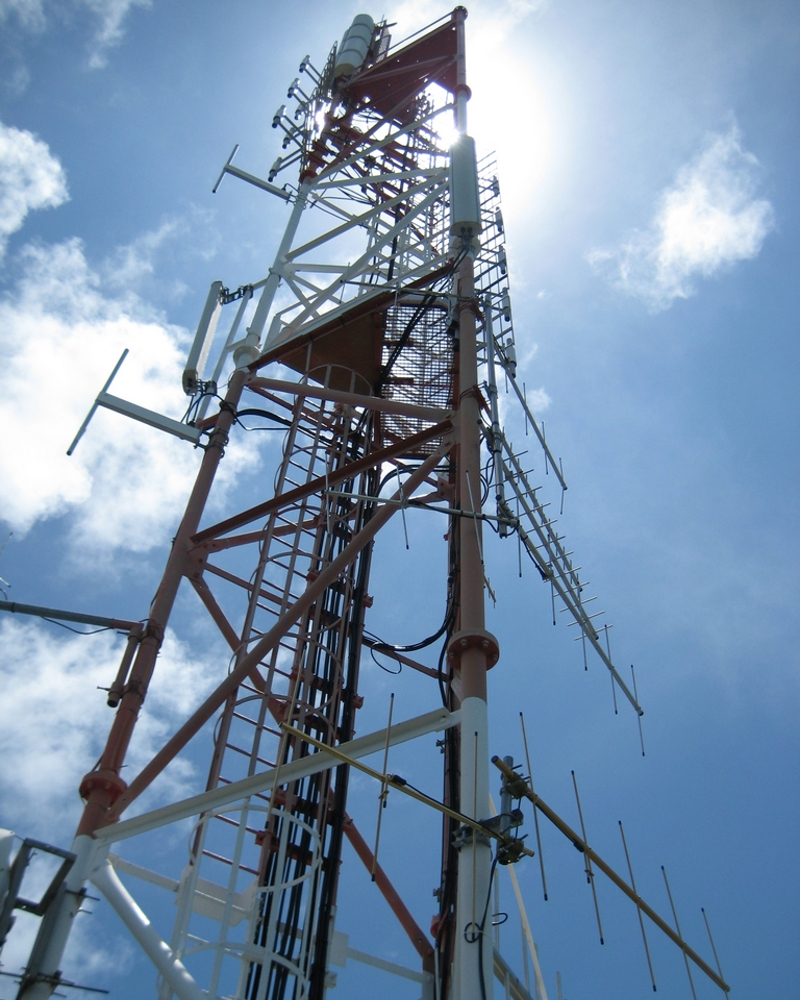
\includegraphics[width=.7\columnwidth]{img/radio.jpg}
      \end{figure}
      \begin{footnotesize}
      \textbf{Onde radio:} $ 10 \, km - 10 \, cm $\\
      Le onde più lunghe di $ 10 \, m $ sono riflesse dalla ionosfera e possono superare la curvatura terrestre.
      \end{footnotesize}
    \end{column}
    \begin{column}{0.3\textwidth}
      \visible<2-3>{\begin{figure}
        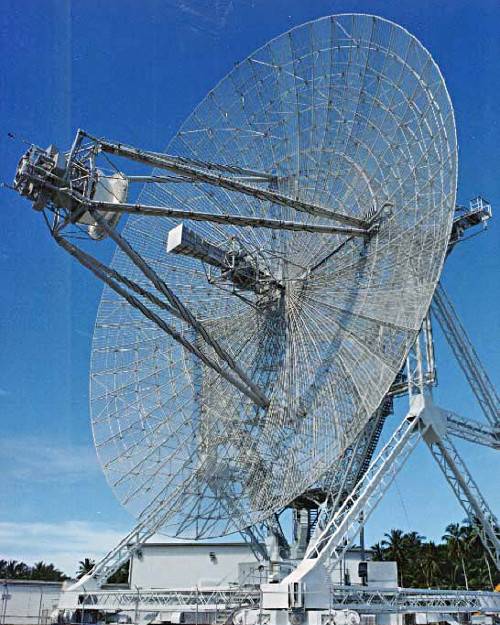
\includegraphics[width=.7\columnwidth]{img/micro.jpg}
      \end{figure}
      \begin{footnotesize}
      \textbf{Microonde:} $ 10 \, cm - 1 \, mm $\\
      Sono usate da cellulari GSM, dai radar, nella comunicazione coi satelliti e nei forni a microonde.
      \end{footnotesize}}
    \end{column}
    \begin{column}{0.3\textwidth}
      \visible<3>{\begin{figure}
        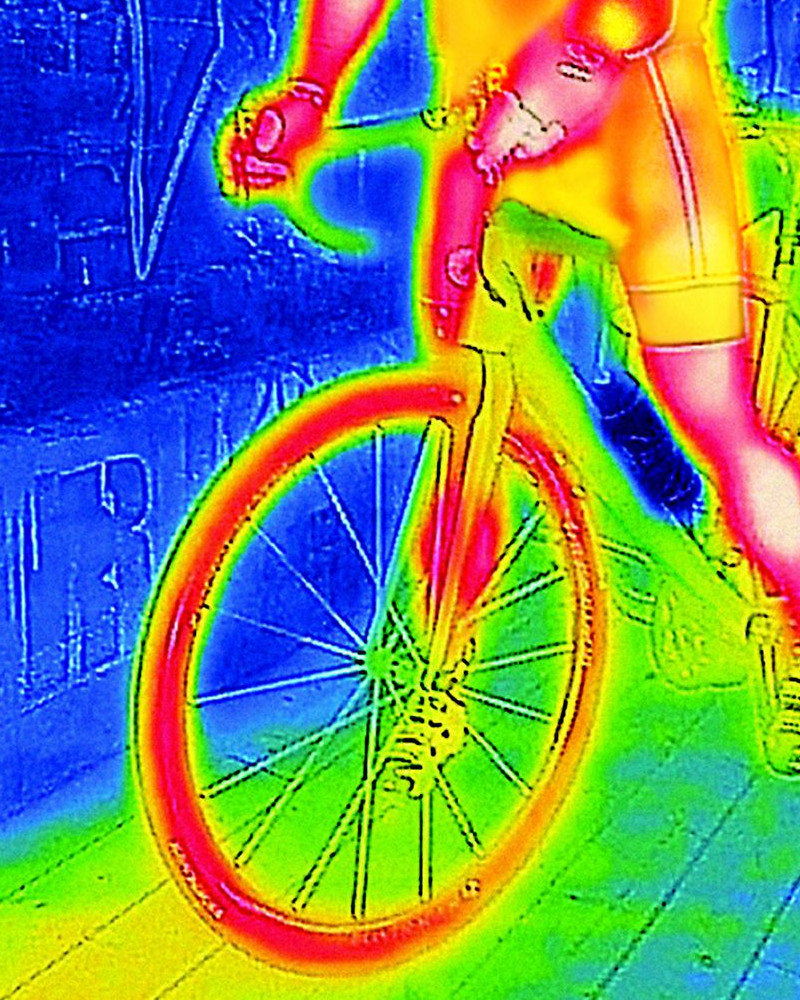
\includegraphics[width=.7\columnwidth]{img/ir.jpg}
      \end{figure}
      \begin{footnotesize}
      \textbf{Radiazione infrarossa:} $ 1 \, mm - 7 \times 10^{-7} \, m $\\
      La percepiamo  come calore ed è usata per la termografia, per la visione notturna e nei telecomandi.
      \end{footnotesize}}
    \end{column}

  \end{columns}
\end{frame}


\begin{frame}
\frametitle{Tipi di onde (2)}
  \begin{columns}
    \begin{column}{0.3\textwidth}
      \begin{figure}
        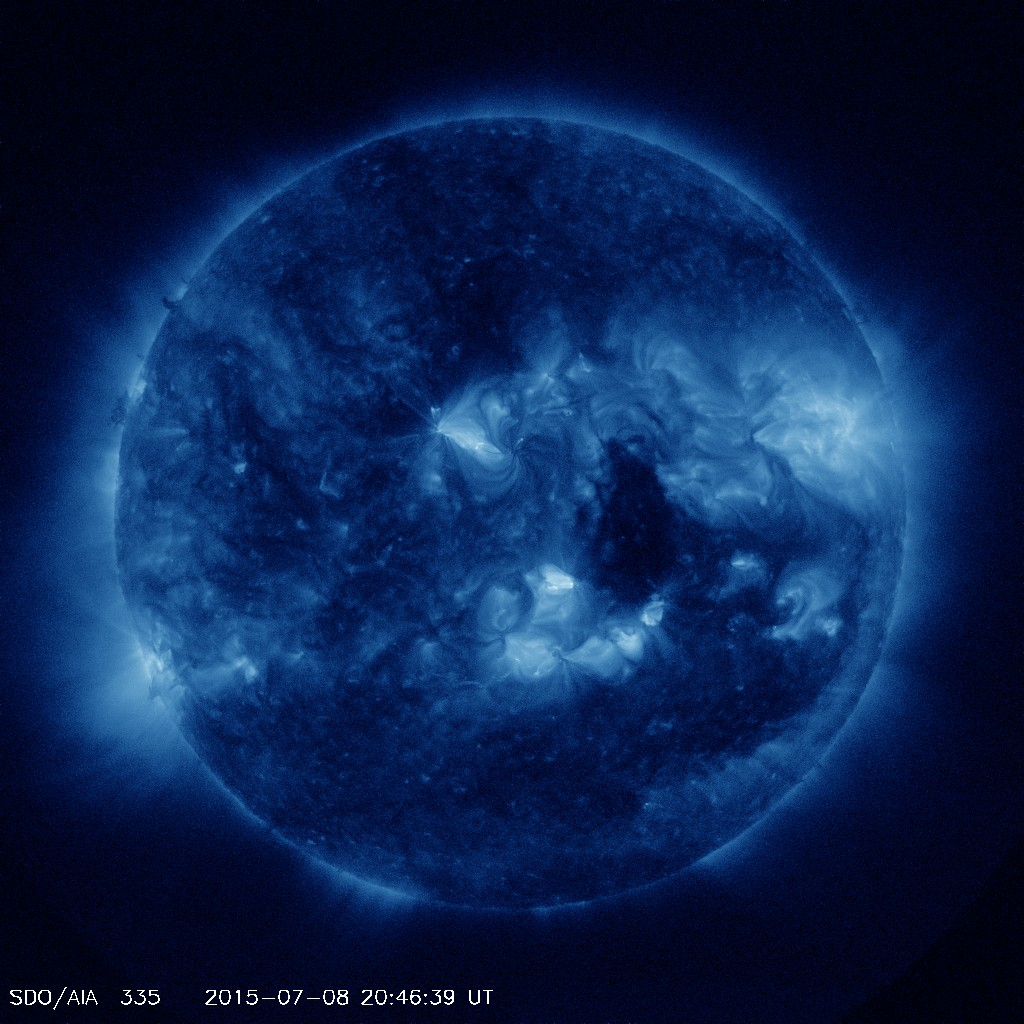
\includegraphics[width=.8\columnwidth]{img/uv.jpg}
      \end{figure}
      \begin{footnotesize}
      \textbf{Raggi ultravioletti:} $ 4 \times 10^{-7} \, m - 1 \times 10^{-8} \, m $\\
      Favoriscono la produzione di melanina nel corpo (non esagerare!) e sono usati in astronomia.
      \end{footnotesize}
    \end{column}
    \begin{column}{0.3\textwidth}
      \visible<2-3>{\begin{figure}
        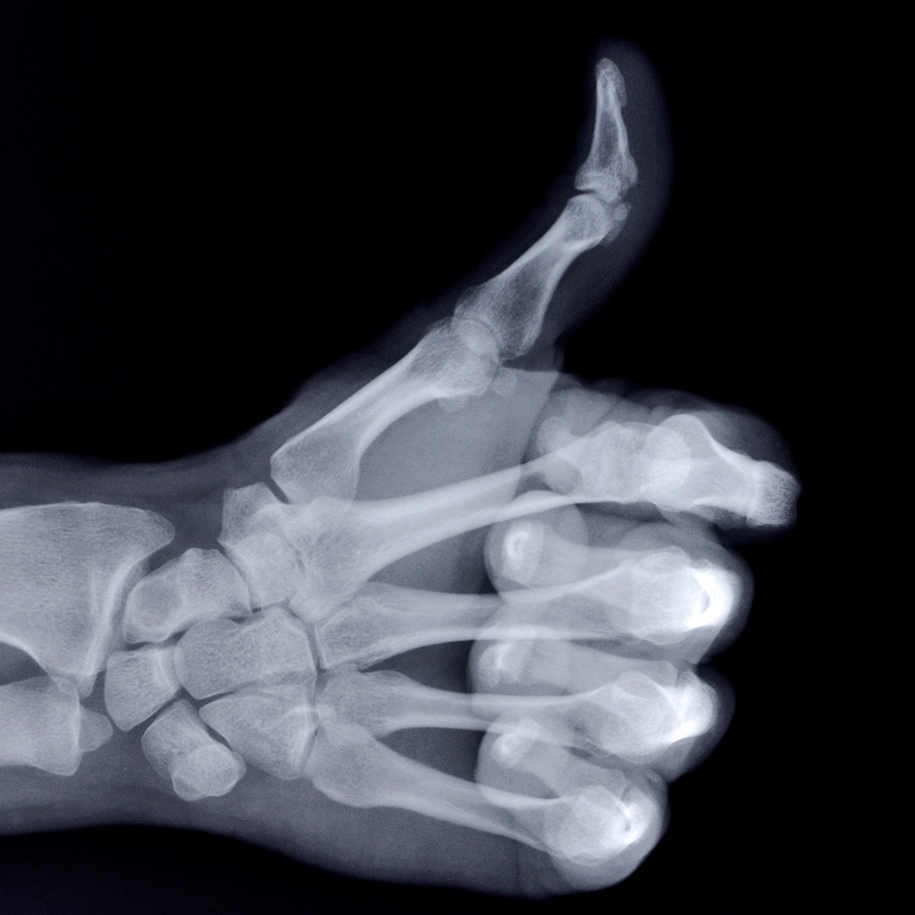
\includegraphics[width=.8\columnwidth]{img/x.jpg}
      \end{figure}
      \begin{footnotesize}
      \textbf{Raggi X:} $ 1 \times 10^{-8} \, m - 1 \times 10^{-11} \, m $\\
      Attraversano i tessuti molli del corpo, ma sono arrestati dalle ossa, usati per le radiografie.
      \end{footnotesize}}
    \end{column}
    \begin{column}{0.3\textwidth}
      \visible<3>{\begin{figure}
        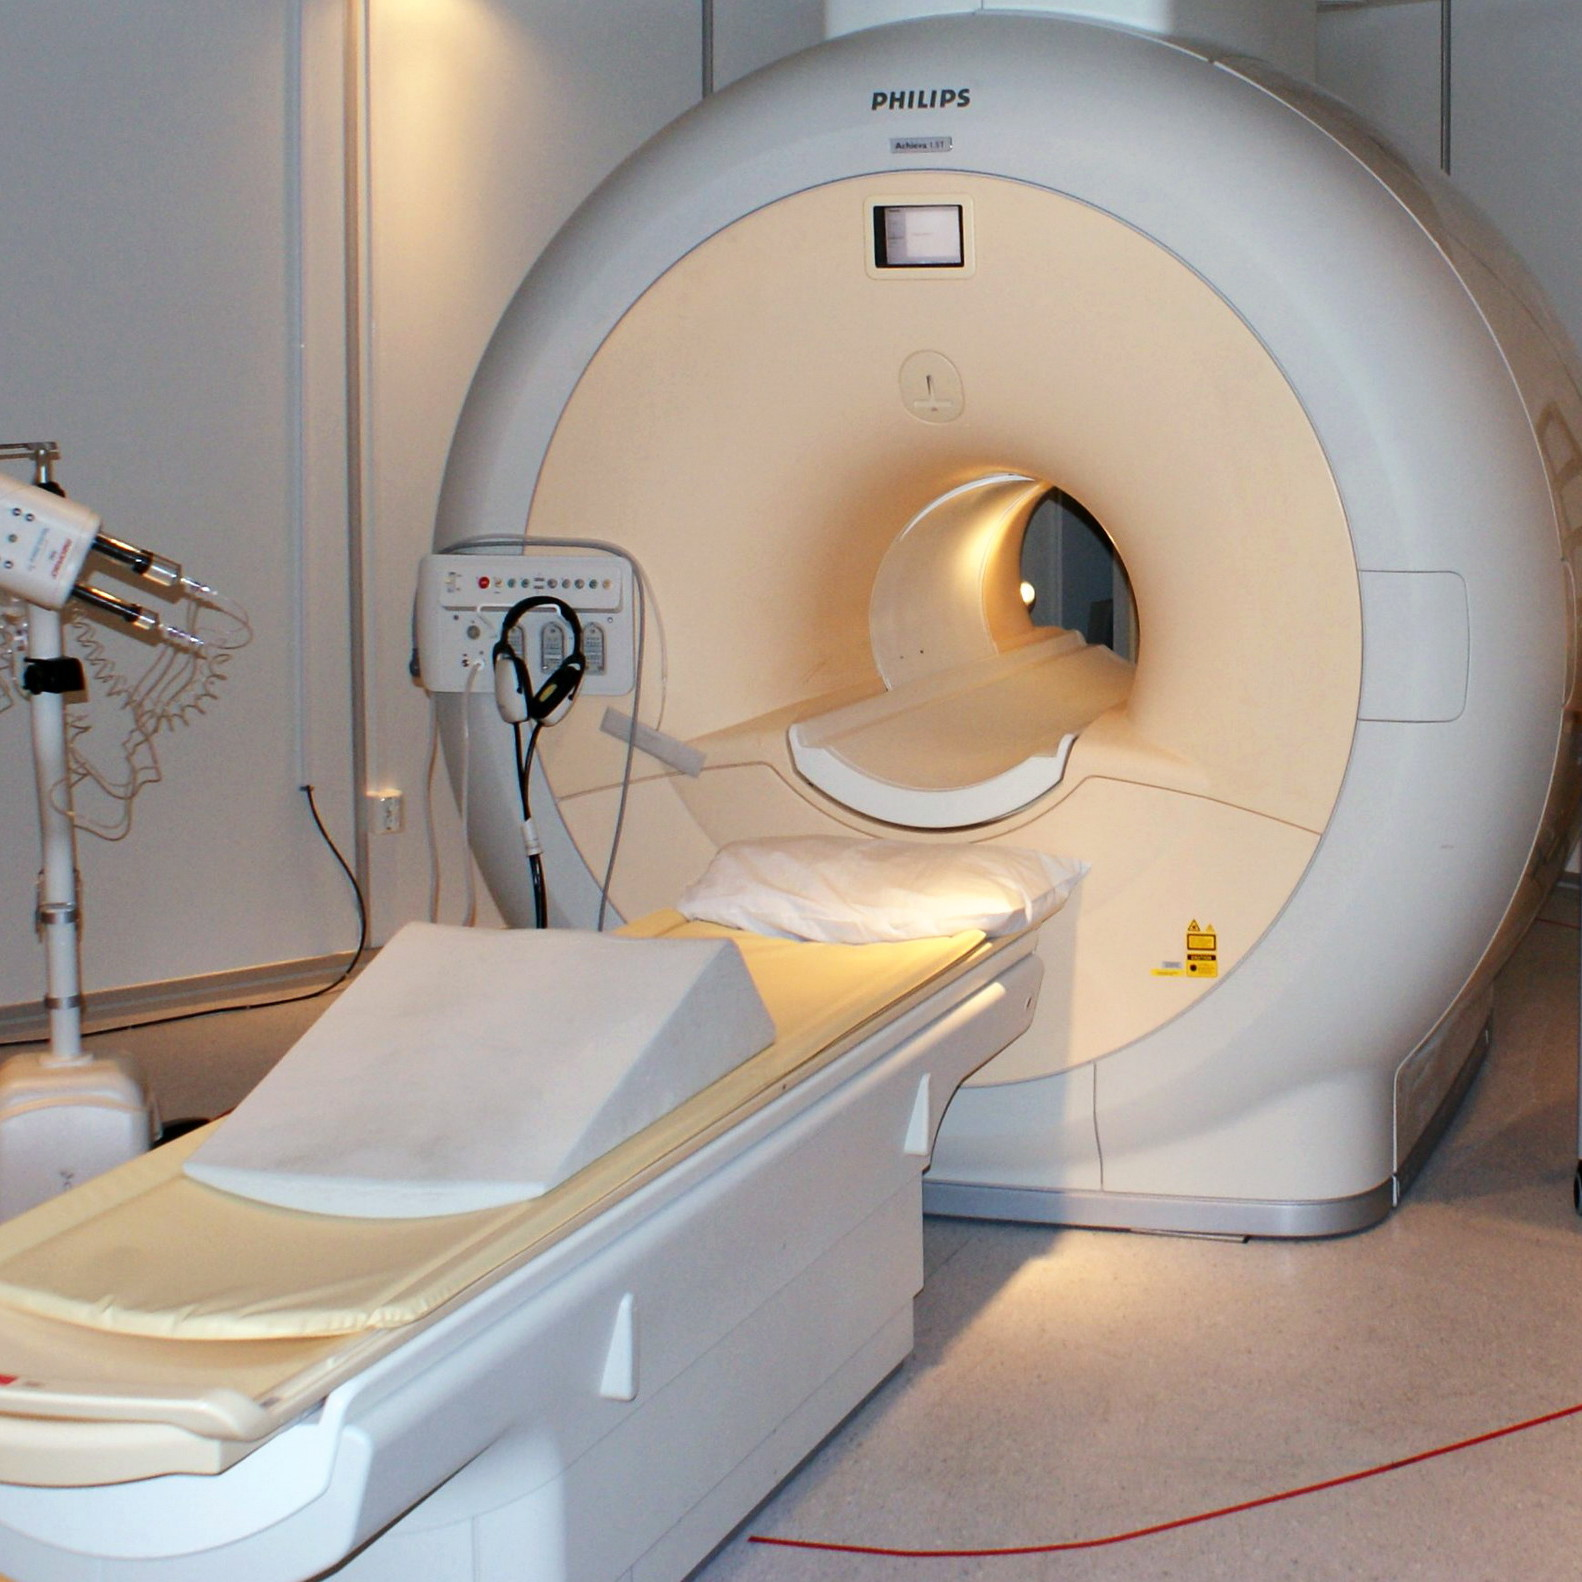
\includegraphics[width=.8\columnwidth]{img/gamma.jpg}
      \end{figure}
      \begin{footnotesize}
      \textbf{Raggi gamma:} $ < 1 \times 10^{-12} \, m $\\
      Accompagnano fenomeni di radioattività e reazioni nucleari, utilizzati in radioterapia.
      \end{footnotesize}}
    \end{column}

  \end{columns}
\end{frame}





%sezione su polarizzazione ecc

%
% \section{Problemi}
%
% \begin{frame}
% Osservazioni generali sulle equazioni, chiudono il cerchio
%
% problema dell'invarianza di c
% \end{frame}
%

\end{document}
